%!TEX root = ../vortrag.tex
\section{Klassifizierung mit Locality-constrained Linear Coding, Spatial Pyramid Matching und linearen SVMs}
\begin{frame}[t,fragile]{Übersicht}
	\begin{itemize}
		\item Ansatz zur Klassifizierung von \citet{lsp06}
		\item ursprünglich zur Klassifikation von Szenen benutzt (z.B. Gebirge, Strand, Stadt)
		\item Erweiterung des Bag-of-Words-Ansatzes, bei dem auch die räumliche Anordnung von Features im Bild beachtet wird
		\item Aufbau des Algorithmus:
		\begin{enumerate}
			\item berechne SIFT-Features über zufälligen Bildausschnitten und clustere sie in Codebook
			\item berechne für jedes Eingabebild dichte SIFT-Features in Spatial Pyramid
			\item wende Locality-constrained Linear Coding (LLC) auf jedem Feature an
			\item poole die LLC-Codes aus jedem Spatial Bin
			\item konkateniere alle gepoolten Codes der Spatial Pyramid
			\item normalisiere diese konkatenierten Codes
			\item trainiere damit eine Support Vector Machine mit linearem Kernel
		\end{enumerate}
	\end{itemize}
\end{frame}

\begin{frame}[t, fragile]{Spatial Pyramid}
	\begin{figure}
		\centering
		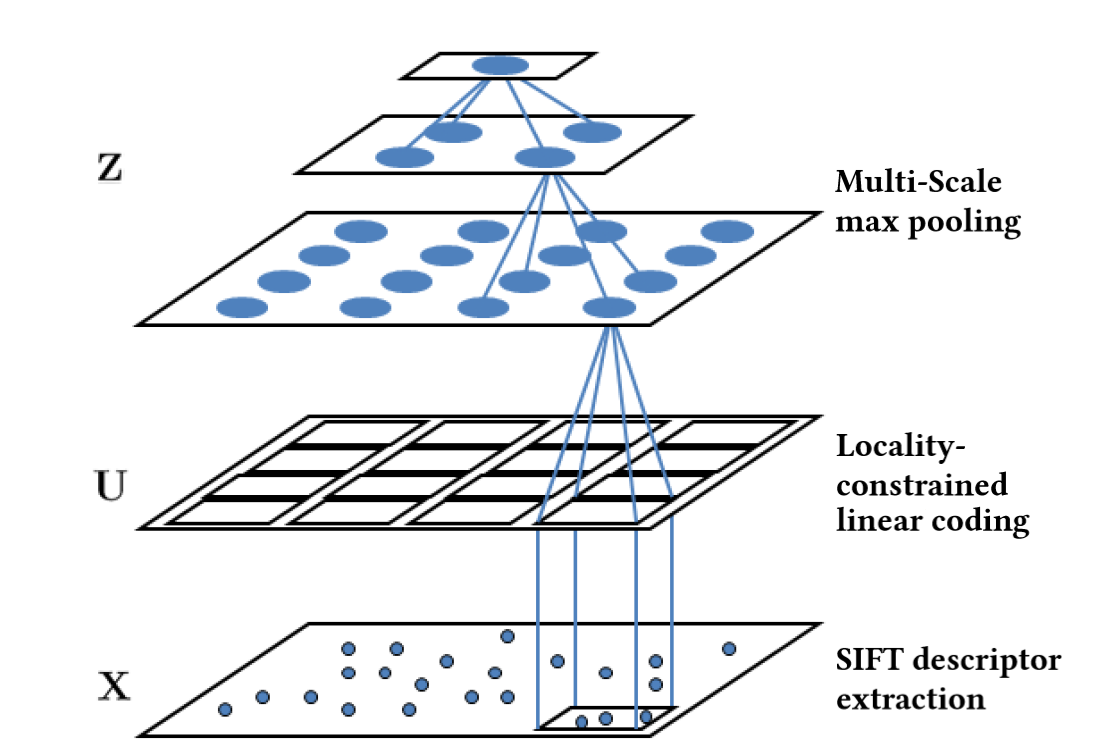
\includegraphics[scale=0.25]{img/architecture}
		\caption{Architektur des Spatial-Pyramid-Matching-Ansatzes \cite{yygh09}}
	\end{figure}
\end{frame}

\begin{frame}[t, fragile]{Locality-constrained Linear Coding (LLC)}
	\begin{figure}
		\centering
		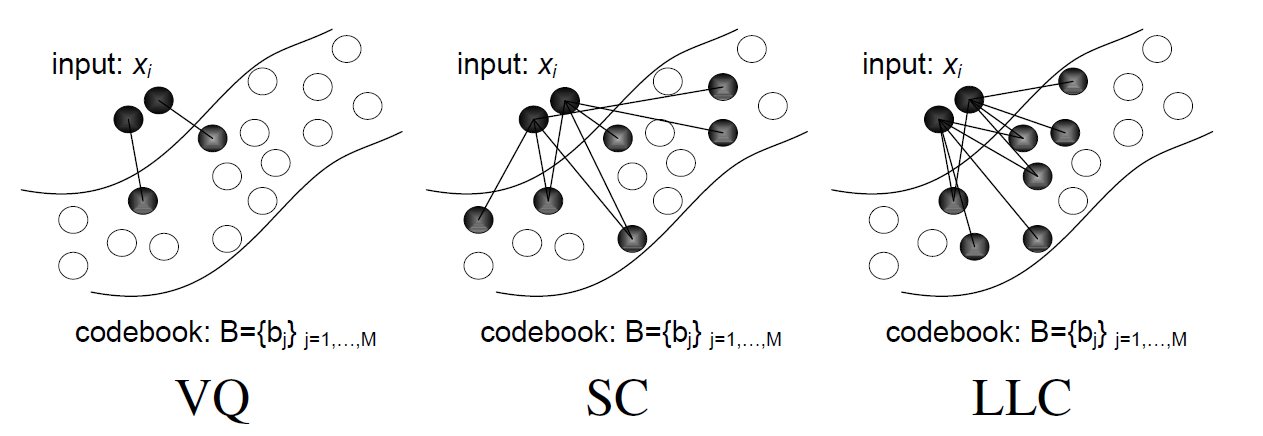
\includegraphics[scale=0.7]{img/quant_comp.png}
		\caption{Vergleich verschiedener Quantisierungsstrategien \cite{wyylhg10}}
	\end{figure}
\end{frame}

\begin{frame}[t, fragile]{Locality-constrained Linear Coding (LLC) II}
	\begin{itemize}
		\item Gegeben D-dimensionale Features $X = [x_1, \dots, x_N] \in \mathbb{R}^{(D \times N)}$ und Codebook mit M Einträgen $B = [b_1, \dots, b_M] \in \mathbb{R}^{(D \times M)}$. 
		\item Gesucht: lokale Zuordnung $C = [c_1, \dots, c_N] \in \mathbb{R}^{(M \times N)}$, die Features aus $X$ Visual Words aus $B$ zuweist  
	\end{itemize}	 
	\begin{equation}
		\min_C \sum_{i=1}^{N} ||x_i - B\cdot c_i||^2 + \lambda\cdot ||d_i \odot c_i||^2, \text{ s.t. } 1^Tc_i = 1 \forall i
	\end{equation}
	\begin{itemize}
		\item Hierbei ist $\odot$ die elementweise Multiplikation und $d_i$ ist ein Distanzterm, der die Ähnlichkeit von Feature $x_i$ zu allen Visual Words des Codebooks wiederspiegelt.
	\end{itemize}
	\begin{equation}
		d_i = \exp \left( \frac{ \mathop{dist}(x_i, B)}{\sigma} \right)
	\end{equation}
\end{frame}

\begin{frame}[t, fragile]{Analytische Lösung von LLC}
	\begin{itemize}
		\item Anders als viele andere Quantisierungsstrategien lässt sich LLC analytisch lösen.
		\begin{itemize}
			\item wir können selber etwas programmieren
			\item (angeblich) in der Praxis schneller
		\end{itemize}
	\end{itemize}
	\begin{equation*}
		\text{ber. Kovarianzmatrix } C_i = (B-1x_i^T)(B-1x_i^T)^T
	\end{equation*}
	\begin{equation}
		\text{Löse LGS: } (C_i + \lambda\mathop{diag}(d_i)) \cdot \tilde{c}_i = (1, \dots, 1)^T
	\end{equation}
	\begin{equation}
	\text{Normalisiere: } c_i = \frac{\tilde{c}_i}{1^T\tilde{c}}
	\end{equation}
\end{frame}

\begin{frame}[t, fragile]{Pooling und Normalisierung}
	\begin{itemize}
		\item poole die LLC-Codes für jeden Spatial Bin:
		\begin{itemize}
			\item sum pooling: $c_{out} = c_1 + \dots + c_N$
			\item max pooling: $c_{out} = \max(c_1, \dots, c_N)$
		\end{itemize}
		\item konkateniere die gepoolten LLC-Codes für jeden Spatial Bin:
		\begin{itemize}
			\item insgesamt 21 konkatenierte LLC-Codes (Level 0: 1, Level 1: 4, Level 2: 16)
		\end{itemize}
		\item normalisiere die konkatenierten Codes:
		\begin{itemize}
			\item sum normalization: $c_{out} = c_{in} / \sum_{j}c_{in}(j)$
			\item $\mathit{l}^2$ normalization: $c_{out} = c_{in} / ||c_{in}||_2$
		\end{itemize}
		\item in der Praxis haben sich Max-Pooling und $\mathit{l}^2$-Normalisierung durchgesetzt \cite{wyylhg10}
	\end{itemize}
\end{frame}

\begin{frame}[t, fragile]{Support Vector Machine mit linearem Kernel}
	\begin{itemize}
		\item Empirische Tests haben ergeben, dass Spatial-Pyramid-Matching-Codes gut linear separierbar sind und diese bessere Ergebnisse liefern als nicht-lineare Kernel \cite{lsp06}.
		\item Benutze Support Vector Machine mit linearem Kernel $k(z_i, z_j) = z_i^Tz_j$ und \emph{quadratic hinge loss}-Funktion.
		\begin{itemize}
			\item Training in $\oh(N)$ und Testen in $\oh(1)$ statt $\oh(N^3)$ und $\oh(N)$ für nicht-lineare Mercer-Kernel.
		\end{itemize}
	\end{itemize}
\end{frame}

\begin{frame}[t, fragile]{Umsetzung}
	\begin{itemize}
		\item Programmiersprache Python
		\item größtenteils mit \emph{numpy} umgesetzt
		\item Parallelisierung der Enkodierung von Level 2 Spatial Bins mit Pythons Multiprocessing
		\item Berechnung der SIFT-Features mit OpenCV
		\item Clustering für Codebook mit Scikit-learns \emph{MiniBatchKMeans} \cite{sklearn}
		\begin{itemize}
			\item deutlich schnellere Laufzeit als \emph{KMeans}
			\item identische Ergebnisse
		\end{itemize}
		\item Scikit-Learns \emph{LinearSVC} als Support Vector Machine \cite{sklearn}
		\begin{itemize}
			\item setzt linearen Kernel und quadratische Hinge-Loss-Funktion schon um
			\item effizienter als SVC(kernel='linear')
		\end{itemize}
	\end{itemize}
\end{frame}